\begin{figure}
  \centering
%  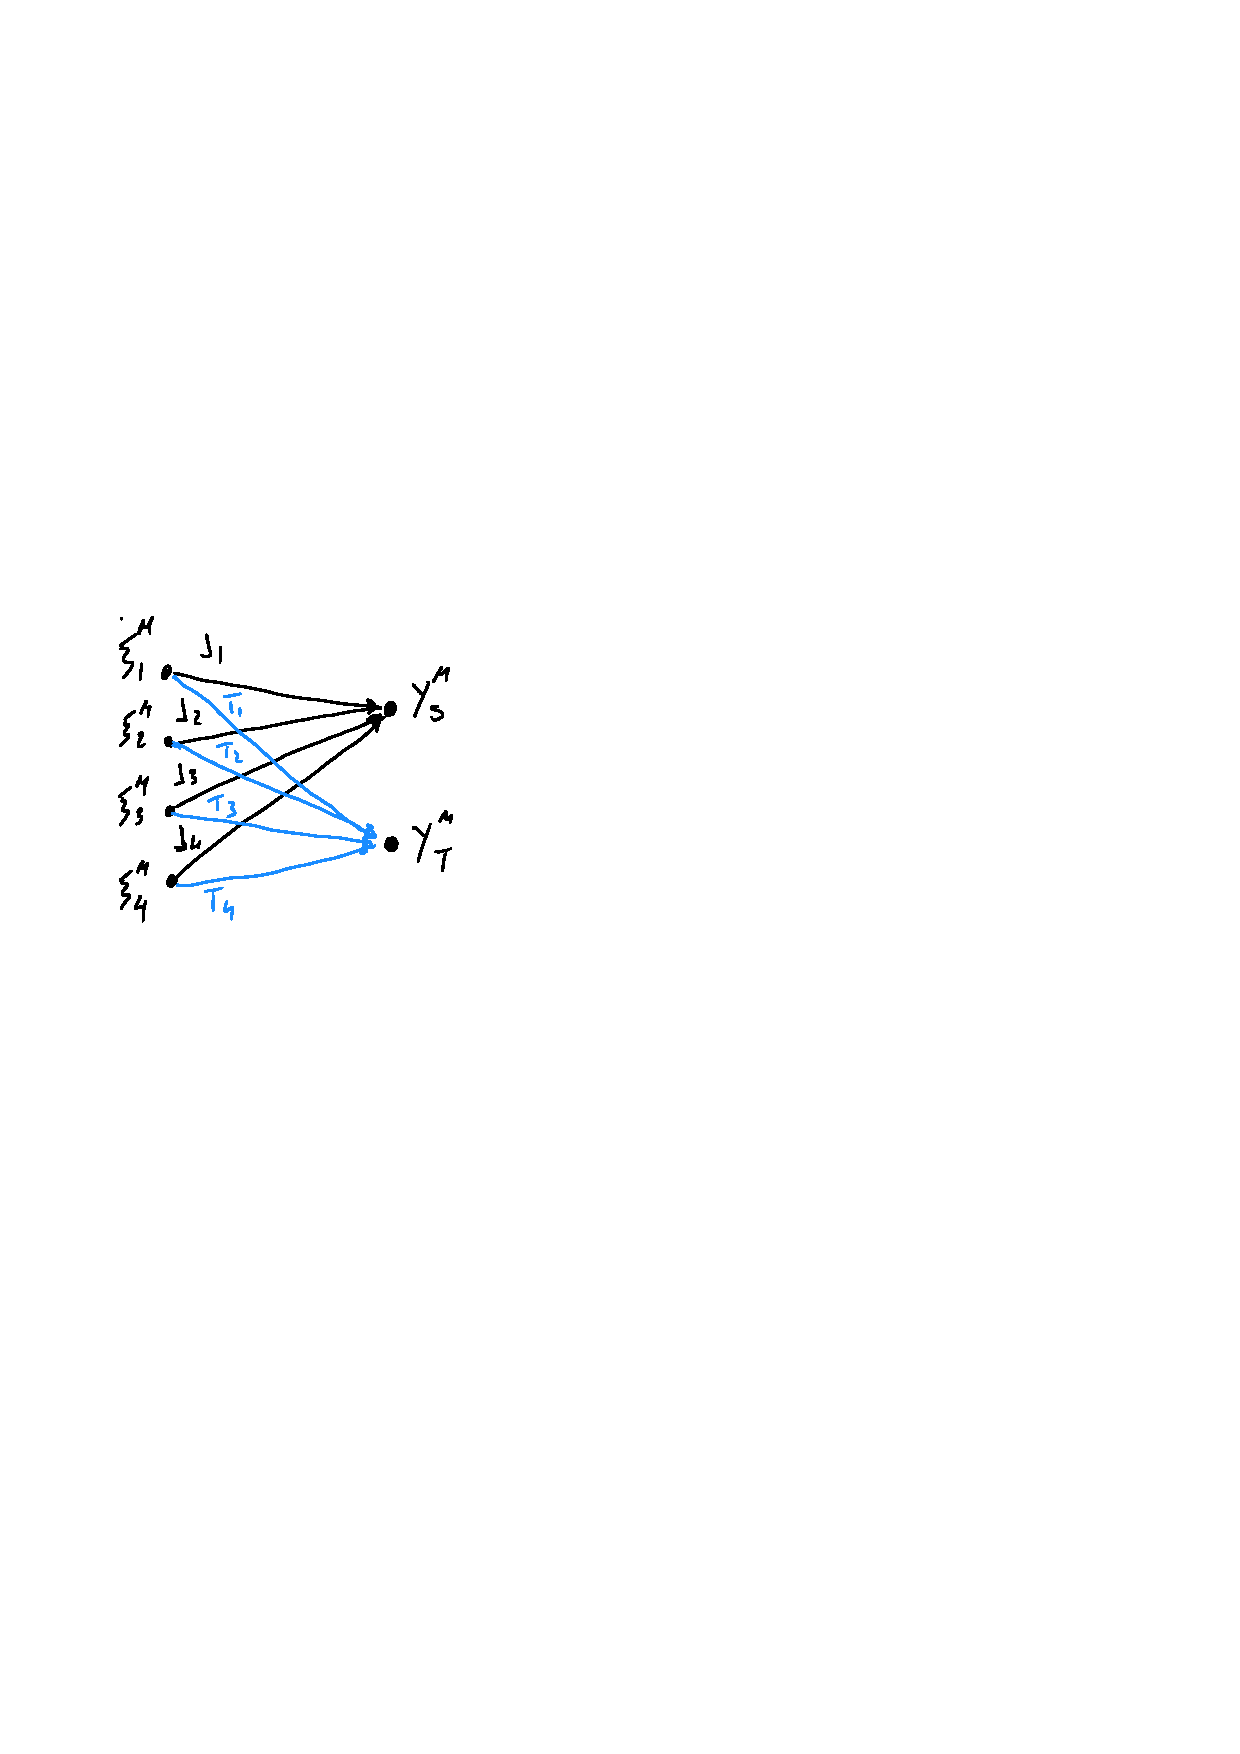
\includegraphics[width = 0.3\textwidth]{./img/perceptron.pdf}
  \begin{center}
  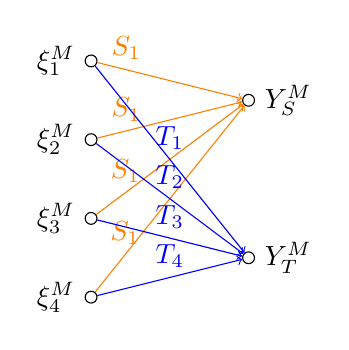
\begin{tikzpicture}
    \node[draw, circle, minimum size=0.15cm, inner sep=0.05cm] (A) at (0, 3) {};
    \node[draw, circle, minimum size=0.15cm, inner sep=0.05cm] (B) at (0, 2) {};
    \node[draw, circle, minimum size=0.15cm, inner sep=0.05cm] (C) at (0, 1) {};
    \node[draw, circle, minimum size=0.15cm, inner sep=0.05cm] (D) at (0, 0) {};

    \node[left] at (A.west) {$\xi_1^M$};
    \node[left] at (B.west) {$\xi_2^M$};
    \node[left] at (C.west) {$\xi_3^M$};
    \node[left] at (D.west) {$\xi_4^M$};

    \node[draw, circle, minimum size=0.15cm, inner sep=0.05cm] (Y) at (2, 2.5) {};
    \node[draw, circle, minimum size=0.15cm, inner sep=0.05cm] (Z) at (2, 0.5) {};

    \node[right] at (Y.east) {$Y_S^M$};
    \node[right] at (Z.east) {$Y_T^M$};
  
    % Arrows
    \draw[->, orange] (A) -- (Y) node[pos=0.2, above] {$S_1$};
    \draw[->, orange] (B) -- (Y) node[pos=0.2, above] {$S_1$};
    \draw[->, orange] (C) -- (Y) node[pos=0.2, above] {$S_1$};
    \draw[->, orange] (D) -- (Y) node[pos=0.2, above] {$S_1$};

    \draw[->, blue] (A) -- (Z) node[pos=0.5, above] {$T_1$};
    \draw[->, blue] (B) -- (Z) node[pos=0.5, above] {$T_2$};
    \draw[->, blue] (C) -- (Z) node[pos=0.5, above] {$T_3$};
    \draw[->, blue] (D) -- (Z) node[pos=0.5, above] {$T_4$};

  \end{tikzpicture}
  \end{center}
  \caption{Pictorial representation Student and Teacher Perceptrons.}
\end{figure}

